\documentclass[onecolumn, draftclsnofoot,10pt, compsoc]{IEEEtran}
\usepackage{graphicx}
\usepackage{url}
\usepackage{setspace}
\usepackage{listings}
\usepackage{float}

\usepackage{geometry}
\geometry{textheight=9.5in, textwidth=7in}

% 1. Fill in these details
\def \CapstoneTeamName{Transportation Modeling}
\def \CapstoneTeamNumber{43}
\def \GroupMemberOne{Eytan Brodsky}
\def \GroupMemberTwo{Liang Du}
\def \GroupMemberThree{Samantha Estrada}
\def \GroupMemberFour{Shengjun Gu}
\def \GroupMemberFive{Charles Koll}
\def \CapstoneProjectName{Autonomous vehicle routing in congested transportation network.}
\def \CapstoneSponsorCompany{Oregon State University}
\def \CapstoneSponsorPerson{Haizhong Wang}

% 2. Uncomment the appropriate line below so that the document type works
\def \DocType{Winter Progress Report - Final Draft}

\newcommand{\NameSigPair}[1]{\par
\makebox[2.75in][r]{#1} \hfil 	\makebox[3.25in]{\makebox[2.25in]{\hrulefill} \hfill		\makebox[.75in]{\hrulefill}}
\par\vspace{-12pt} \textit{\tiny\noindent
\makebox[2.75in]{} \hfil		\makebox[3.25in]{\makebox[2.25in][r]{Signature} \hfill	\makebox[.75in][r]{Date}}}}
% 3. If the document is not to be signed, uncomment the RENEWcommand below
%\renewcommand{\NameSigPair}[1]{#1}

%%%%%%%%%%%%%%%%%%%%%%%%%%%%%%%%%%%%%%%
\begin{document}
\begin{titlepage}
    \pagenumbering{gobble}
    \begin{singlespace}
        %\includegraphics[height=4cm]{coe_v_spot1}
        \hfill
        % 4. If you have a logo, use this includegraphics command to put it on the coversheet.
        %\includegraphics[height=4cm]{CompanyLogo}
        \par\vspace{.2in}
        \centering
        \scshape{
            \huge CS Capstone \DocType \par
            {\large\today}\par
            \vspace{.5in}
            \textbf{\Huge\CapstoneProjectName}\par
            \vfill
            {\large Prepared for}\par
            \Huge \CapstoneSponsorCompany\par
            \vspace{5pt}
            {\Large\NameSigPair{\CapstoneSponsorPerson}\par}
            {\large Prepared by }\par
            Group\CapstoneTeamNumber\par
            % 5. comment out the line below this one if you do not wish to name your team
            \CapstoneTeamName\par
            \vspace{5pt}
            {\Large
                \NameSigPair{\GroupMemberOne}\par
                \NameSigPair{\GroupMemberTwo}\par
                \NameSigPair{\GroupMemberThree}\par
                \NameSigPair{\GroupMemberFour}\par
                \NameSigPair{\GroupMemberFive}\par
            }
            \vspace{20pt}
        }
        \begin{abstract}
        % 6. Fill in your abstract
            The purpose of this document is to detail the progress made in the project during Winter term.
            This document discusses overall progress of the project, along with problems and solutions.
        \end{abstract}
    \end{singlespace}
\end{titlepage}
\newpage
\pagenumbering{arabic}
\tableofcontents
% 7. uncomment this (if applicable). Consider adding a page break.
%\listoffigures
%\listoftables
\clearpage

% 8. now you write!
\section{Overview and Goals}
The transportation modeling project models the actions of connected autonomous vehicles at various market penetrations in a transportation network. We build a simulation that has vehicles move about on a grid-like network of roads and intersections. They optimize their routes to their destinations. For the connected autonomous vehicles, they optimize their routes with neural networks that are restrained during every new route. They can connect with other connected autonomous vehicles within a given radius to retrieve additional information to improve their decision-making. The goal of the project is to identify a routing algorithm that makes the simulated vehicles’ actions resemble those of vehicles in the real world. A concise set of data is also expected to be produced, providing a support for our hypothesis that connected autonomous vehicle integration is beneficial for transportation congestion.
\section{Completion}
We have finished the visualization of the vehicles on the transportation network. The Python backend is connected to the JavaScript frontend so that the frontend can pass initialization data from the user to the backend to be used as parameters for the simulation. The frontend can then take the data generated from the backend and render it to the browser so that the user can see it. The work that still needs to be completed is implementing the Intelligent Driver Model (IDM), which determines the actions of a vehicle as it follows another one. Once that is complete, we will have a working Beta version of the code so that the only parts remaining are beautifying the user experience and fixing bugs.
\section{Implementation}
We used two-dimensional plane axes to simulate our test map. In this way, we can let the vehicle or the system determine its current position through the horizontal and vertical coordinates so that the vehicle can take action. In our structure there are three main components: intersection, road, and vehicle. The intersection simulation contains the current coordinate information of the intersection, the number of roads contained by the intersection, and the road information. After that, we will add traffic lights to the intersections. This allows the vehicle to make its own road choices to save time or calculate shortest paths. This is the code for initializing intersections:
\begin{lstlisting}[language=Python]
def init_intersections(self):
    """Initialize intersections"""
    return [
        Intersection(item['id'],
                     item['connects_roads'],
                     (item['loc']['x'], item['loc']['y']))
        for item in self.gui.infrastructure['intersections']
    ]
\end{lstlisting}
For road simulation, each road contains its own starting and ending two-dimensional coordinates. Both the start and end coordinates have intersection coordinates that match. Each road is set to be two-way. Each road has only two lines and has its own "road id", which will help us quickly identify which road has a problem during the test. Road simulations with intersections will help us simulate truly complex urban roads. This is the code for initializing roads:
\begin{lstlisting}[language=Python]
def init_roads(self, intersections):
    """Initialize roads"""
    roads = []
    for item in self.gui.infrastructure['roads']:
        ends = [item['ends'][0], item['ends'][1]]
        # Convert road endpoints to tuples if they're coordinates
        for i in range(2):
            try:
                ends[i] = (ends[i]['x'], ends[i]['y'])
            except TypeError:
                for intersection in intersections:
                    if intersection.intersection_id == ends[i]:
                        ends[i] = intersection
                        break
        roads.append(Road(item['id'], item['two_way'],
                          item['lanes'], (ends[0], ends[1])))
    return roads
\end{lstlisting}
For vehicle simulation, each vehicle has its own vehicle "id", vehicle type, vehicle location coordinates, and vehicle destination coordinates. Each vehicle has its own unique id. For vehicle types, we distinguish between autonomous vehicles and human vehicles. In the following design, we will allow autonomous vehicles to transmit information, so as to optimize the choice of shortest path for autonomous vehicles. Human-powered vehicles will not be able to connect to each other. Secondly, for the position of vehicles, each vehicle will update its two-dimensional coordinate position in real time. This is the code for initializing vehicles:
\begin{lstlisting}[language=Python]
def init_vehicles(self):
    """Initialize vehicles"""
    for item in self.gui.vehicles:
        if item['type'] == 0:
            vehicle = HV()
        elif item['type'] == 1:
            vehicle = CAV()
        else:
            raise ValueError
        vehicle.id = item['id']
        vehicle.location = (item['start_loc']['x'], item['start_loc']['y'])
        vehicle.destination = (item['end_loc']['x'], item['end_loc']['y'])
        self.new_vehicles.append({'entry': item['entry_time'],
                                  'vehicle': vehicle})
\end{lstlisting}
To figure out vehicles’ moving direction, we used linear function to determine each vehicle’ direction on lanes. Because every roads are two-way, vehicles’ direction judgement is based on the center of vehicles, and check if vehicles are in each lanes range. We used “math.hypot(dx, dy)” function to figure out distance of vehicles’ center and roads’ center. The checking vehicles’ moving direction function will be used when vehicles across each intersections. This is the code of checking vehicles’ direction based on vehicles’ coordinates:
\begin{lstlisting}[language=Python]
def lane_direction(self, loc):
    """Return the angle of the lane at the given location"""
    ends = self.coords()
    dx = ends[1][0] - ends[0][0]
    dy = ends[1][1] - ends[0][1]
    angle = math.atan2(dy, dx)
    calc_eq = dy * (loc[0] - ends[0][0]) - dx * (loc[1] - ends[0][1])
    signed_dist = calc_eq / math.hypot(dx, dy)
    if signed_dist < 0:
        angle = math.atan2(-dy, -dx)
    return math.degrees(angle)
\end{lstlisting}
On the transportation network, every point can be represented by a coordinate, and vehicles just can run on roads. Because of that, we created a function in road class which can check if a coordinates on the map is belong to one of roads we created. Actually, when we make vehicle run, vehicles will be guaranteed on roads, but the check if vehicles on roads function can help we test and debug some functions which adject vehicles’ driving route. The principle of checking vehicles’ location function is to calculate the distance of vehicle’s center and roads’ center and compare to the road’s width. This is the code:
\begin{lstlisting}[language=Python]
def has_point(self, loc):
    """Check if a point is on the road"""
    ends = self.coords()
    for i in range(2):
        d_1 = abs(ends[1][i] - ends[0][i])
        d_2 = abs(ends[1][(i + 1) % 2] - ends[0][(i + 1) % 2])
        if (d_1 >= d_2
                and (ends[0][i] < loc[i] and ends[1][i] < loc[i]
                     or ends[0][i] > loc[i] and ends[1][i] > loc[i])):
            return False
    d_x = ends[1][0] - ends[0][0]
    d_y = ends[1][1] - ends[0][1]
    calc_eq = d_y * (loc[0] - ends[0][0]) - d_x * (loc[1] - ends[0][1])
    dist = abs(calc_eq) / math.hypot(d_x, d_y)
    if dist <= self.lanes * 6:
        return True
    return False
\end{lstlisting}
Our current progress on vehicle routing is a simple implementation of Dijkstra’s algorithm utilizing the information that was sent by the GUI and integrated into our infrastructure class. CAV’s at this point in time are intended to run the Dijkstra’s routing algorithm whenever they approach a new intersection, while HV’s only run the algorithm once and store this path as their static route. We have currently the ability to take the information from the front end and use it viably, and update the vehicle’s position accurately using trigonometric methods to account for vehicle movement at different angles. Currently, we are working on the proper implementation of the Intelligent Driver Model (IDM) to insert functionality for car following, safe deceleration, gap space, and safe approach rate when encountering another vehicle.
\section{Problems and Solutions}
The primary problem that has impeded our progress is the lack of prerequisite knowledge of Python. Only two of the five members of the team used Python before this project. To solve this problem, the group has compiled a set of tutorials and documentation on Python so that the code being written will be standardized. This has worked somewhat, although there is still the occasional mishap that quickly becomes worked out.

When we were doing road simulations, we initially intended to do unlimited road simulations. That is, the intersection can connect up to four roads, but there will be no limit to the number of road lines. And we can also have one-way roads. This is also to be able to more close to the real urban road simulation. But when we're doing traffic light simulations (which allow the road to open or close as specified). We found that the increase in the number of roads would greatly increase the amount of coding, such as simulating traffic lights at intersections with the number of mixed lanes. In combination with the problem of one-way lanes or two-way lanes, we will consider dozens of possible scenarios. At the beginning of the simulation, it was unreasonable to design such a complex simulation. So in order to be able to accurately implement our simulation, we felt limited to the number of lanes. That is, all roads are two-way and there are only two lanes. After the initial simulation is complete, we will extend our code to refine it if time permits.
\section{Beta}
\begin{figure}[H]
\caption{Simulation Interface}
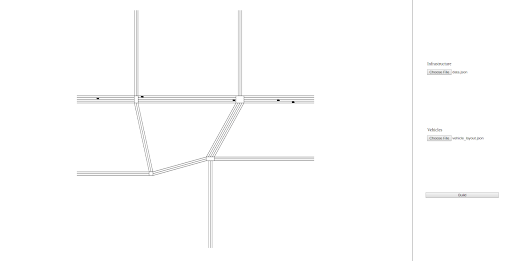
\includegraphics[width=6in]{gui}
\end{figure}
This is our current Beta for the project user interface. The user’s options are fairly limited, only being able to select a road and vehicle layout and play the simulation with no option of pausing. We used json file to store our infrastructures and vehicles’ data. In the “infrastructure” file, it includes intersections and roads’ information. Currently, we considered to change all of road with two lanes because it is easier to handle vehicles’ actions on intersections. For “vehicles” file, it should generate dynamic based on roads’ information. We determined right side lane is “input” road and left side lane is “output” of road on every screen edges. Next, we plan to add more features to the GUI to enable features such as data collection, playbacks and video downloads in the beta and in the finished product. A potential improvement could be to add color to make the interface a little prettier, but that’s not a very urgent issue.
\section{Next Steps}
The next step we're going to do is vehicle following simulation using the IDM. We can show the safety and reliability of autonomous vehicle by vehicle following simulation. For the vehicle following simulation, we will design a data collection system. In the data collection system, we can display the average speed at which vehicles reach their destinations, which includes the different speed of the autonomous vehicle and the human vehicle. By comparing the speeds we can draw some conclusions, such as how much faster an autonomous vehicle can reach its destination than a human vehicle. Although ideally the driving speed of the autonomous vehicle is the same as that of the human vehicle, the average speed of the autonomous vehicle is theoretically better than that of the human vehicle because the autonomous vehicle has the shortest path selection algorithm.

An important part of this project is to give the user insights into statistics in the simulation, such as speed, velocity, averages, extremes, etc… Our application intends to provide this information through graphs and providing the raw data to the user if they choose. The way we have decided to do this is by keeping track of the vehicle’s speeds and positions, from which we can get other data points at the end of the simulation like average speed, average acceleration, average stopping time, etc… and provide streaming data about each vehicle’s speed and acceleration by sending json data from the back end to the front end.
The graph below is not what we intend the application to produce exactly, but gives a rough idea of what one of the basic graphs that the user might be interested in would look like. The graph shows the different speeds achieved by a human-driven vehicle and an autonomous vehicle every second in a simulation. The below example is not real data, but of course different simulations would yield different graphs.
\begin{figure}[H]
\caption{Vehicle Speed Over Time Example}
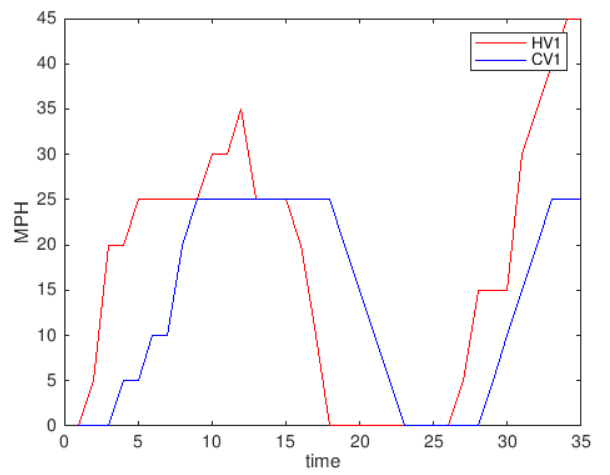
\includegraphics[width=3.5in]{graph}
\end{figure}
\end{document}
